\documentclass{article}
\usepackage{oconnor}
\usepackage{ wasysym }

%% UPDATE these variables:
\renewcommand{\hwnum}{1}
\title{CSCI 446, Project Design 01}
\author{Group 20: Patrick O'Connor, Jack Tetrault, John Hultman}
%%\date{due: 15 January 2021}

\begin{document}

\maketitle

CSCI 446 Artificial Intelligence

Project 01: Sudoku

Elements of Design Document
\begin{enumerate}
    \item UML Class Diagram
    \item Algorithm Design Decisions
    \item Experimental Design for Testing Results
\end{enumerate}
% ============================================
% ============================================
\nextprob{}

% ============================================

\paragraph{UML Class Diagram}

Please note that many of our decisions have been discussed with notes on the side of the class that the note is referencing.

\begin{figure}
    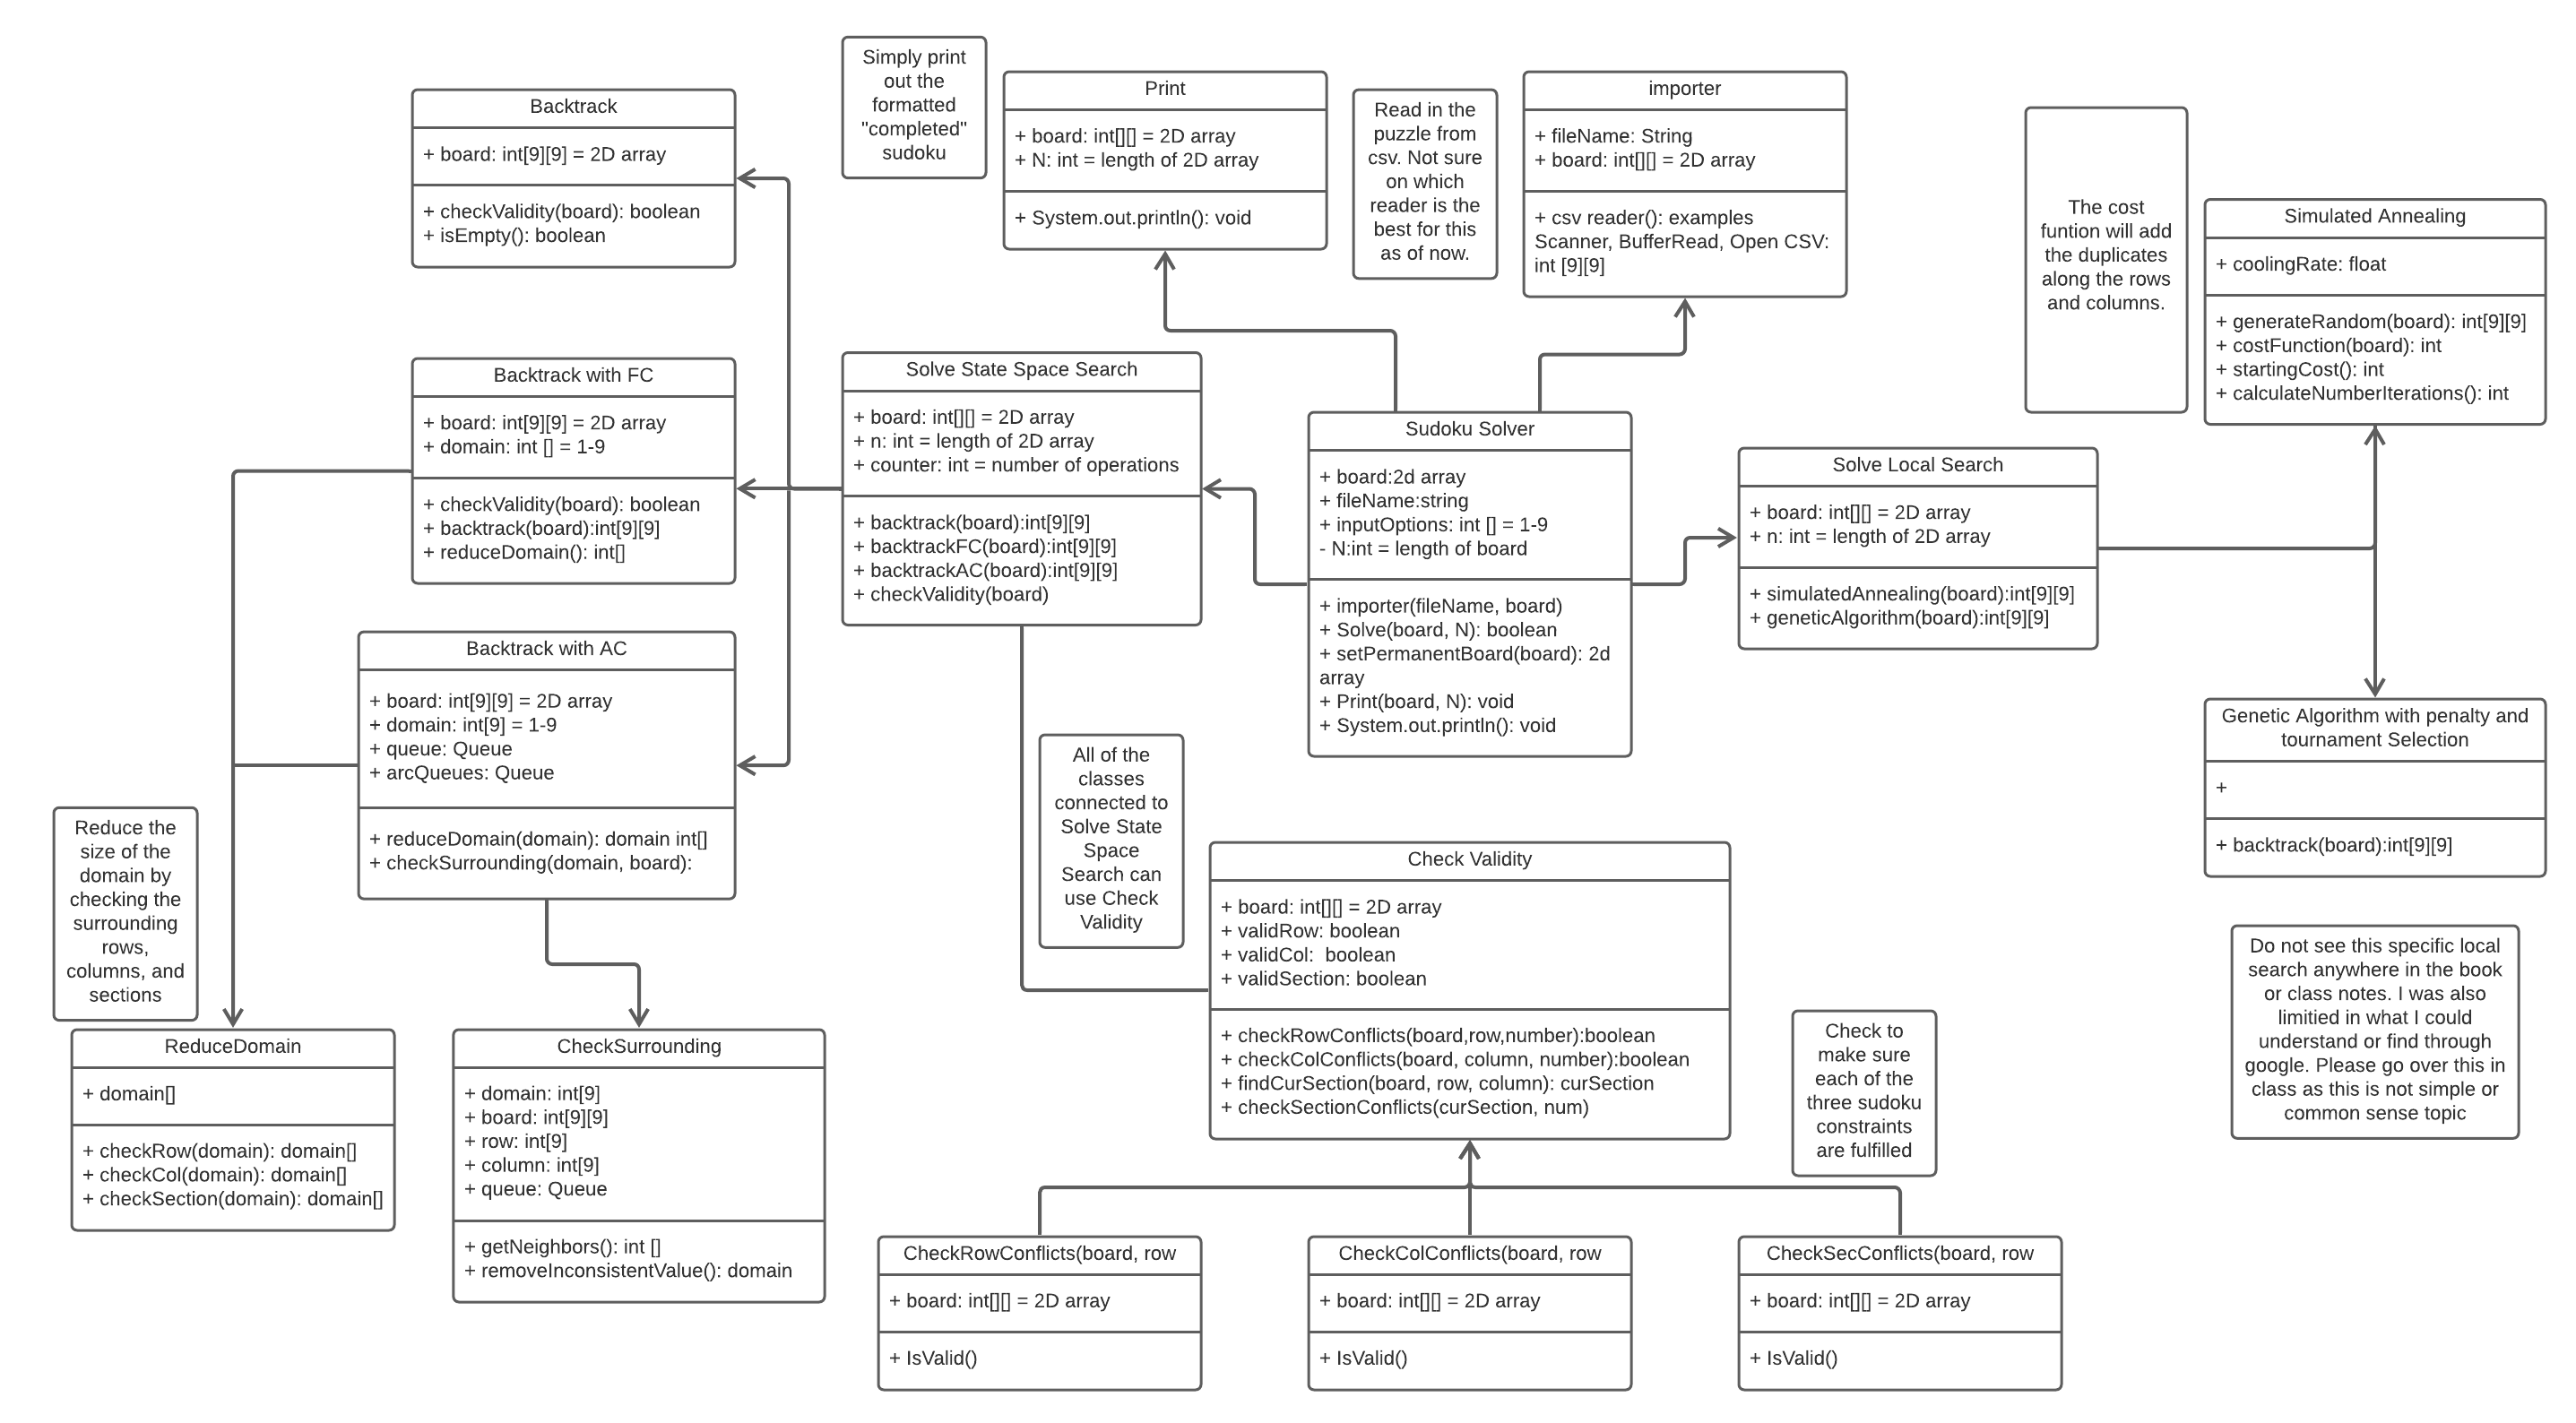
\includegraphics[width=\textwidth]{SudokuUMLDiagram.png}
    \caption{UML Drawn using Lucid App}
    \label{fig:num01}
\end{figure}
See figure \ref{fig:num01} for UML Class Diagram

% ============================================
% ============================================
\nextprob{}
% ============================================

\paragraph{Algorithm Design Decisions}
Our main design decisions were that we broke up our search algorithms into two inheritance classes, 
with the parent classes being stateSpaceSearch and localSearch.  
State space search has three child classes where we will implement standard backtracking, 
backtracking with forward checking, and backtracking with arc consistency.  Local search has 
two child classes where we will implement our two local search algorithms, the simulated annealing class and the genetic algorithm class.


Our other main design decision was that we created an entire class for checking for validity that we 
will use from any of the algorithms to check for conflicting values. 

Both of these design decisions will reduce the complexity of our codebase by creating an entire class that 
can be used multiple times with relatively smalls calls.



\paragraph{Experimental Design for Testing Results}
After researching how the required constraint solvers work, there are a couple of variables that we 
could choose to be our dependent variable. These variables are all pertaining to how fast the 
algorithm/method can achieve the goal of completing the sudoku puzzle. The two most readily available 
and accurately measurable are execution time and computation(”moves”) counters. 

We have decided that the hypothesis that we will be examining is the computation (”moves”) counter. 
Thus our official hypothesis is:

When attempting to complete a sudoku puzzle of varying difficulties which of the following 
listed variations of a constraint solver is the most efficient?

\begin{enumerate}
    \item Simple backtracking (only run this on easy and medium puzzles)
    \item Backtracking with forward checking 
    \item Backtracking with arc consistency 
    \item Local search using simulated annealing with the minimum conflict heuristic 
    \item Local search using a genetic algorithm with a penalty function and tournament selection
\end{enumerate}

In order to, test this hypothesis we will successfully implement each of the variations noted above and 
test them to ensure functionality is correct. After initial testing, the counter will be turned on and each of 
the variations will be ran numerous times on a variety of 20 different sudoku puzzles. Each time the puzzle is completed 
the counter for that respective puzzle will be stored based on approach and puzzle difficulty in a table. After many iterations, 
we will be able to make an educated guess on which of our implementations is the best for each difficulty and in general.

\end{document}

